\section{Versuchsbeschreibung}
\label{section:Versuchsbeschreibung}
%
Der Prüfstand besteht aus einem Wasserkreislauf, angetrieben durch eine Pumpe wird Wasser durch ein Rohrsystem zur zu vermessenen Peltonturbine geleitet.\\
Im Verlauf des Rohrsystems werden sowohl der Druck als auch der Volumenstrom gemessen.
Hierfür werden Drucksensoren vom Typ \textit{PA3526} der Firma \textit{ifm electronic} genutzt, sowie eine Volumenstrommesseinheit.
Diese werden mit je einem Multimeter verschaltet von denen man dann einen Wert in \textit{mA} ablesen kann, welcher in den gesuchten Wert umgerechnet werden kann.\\
Eine Düse komprimiert dann den Wasserstrahl auf die Schaufeln der Peltonturbine.
Der Prüfstand im Stillstand ist ebenfalls in \autoref{fig:Aufbau_Stillstand} zu erkennen.\\
%
\begin{figure}[!h]
    \centering
    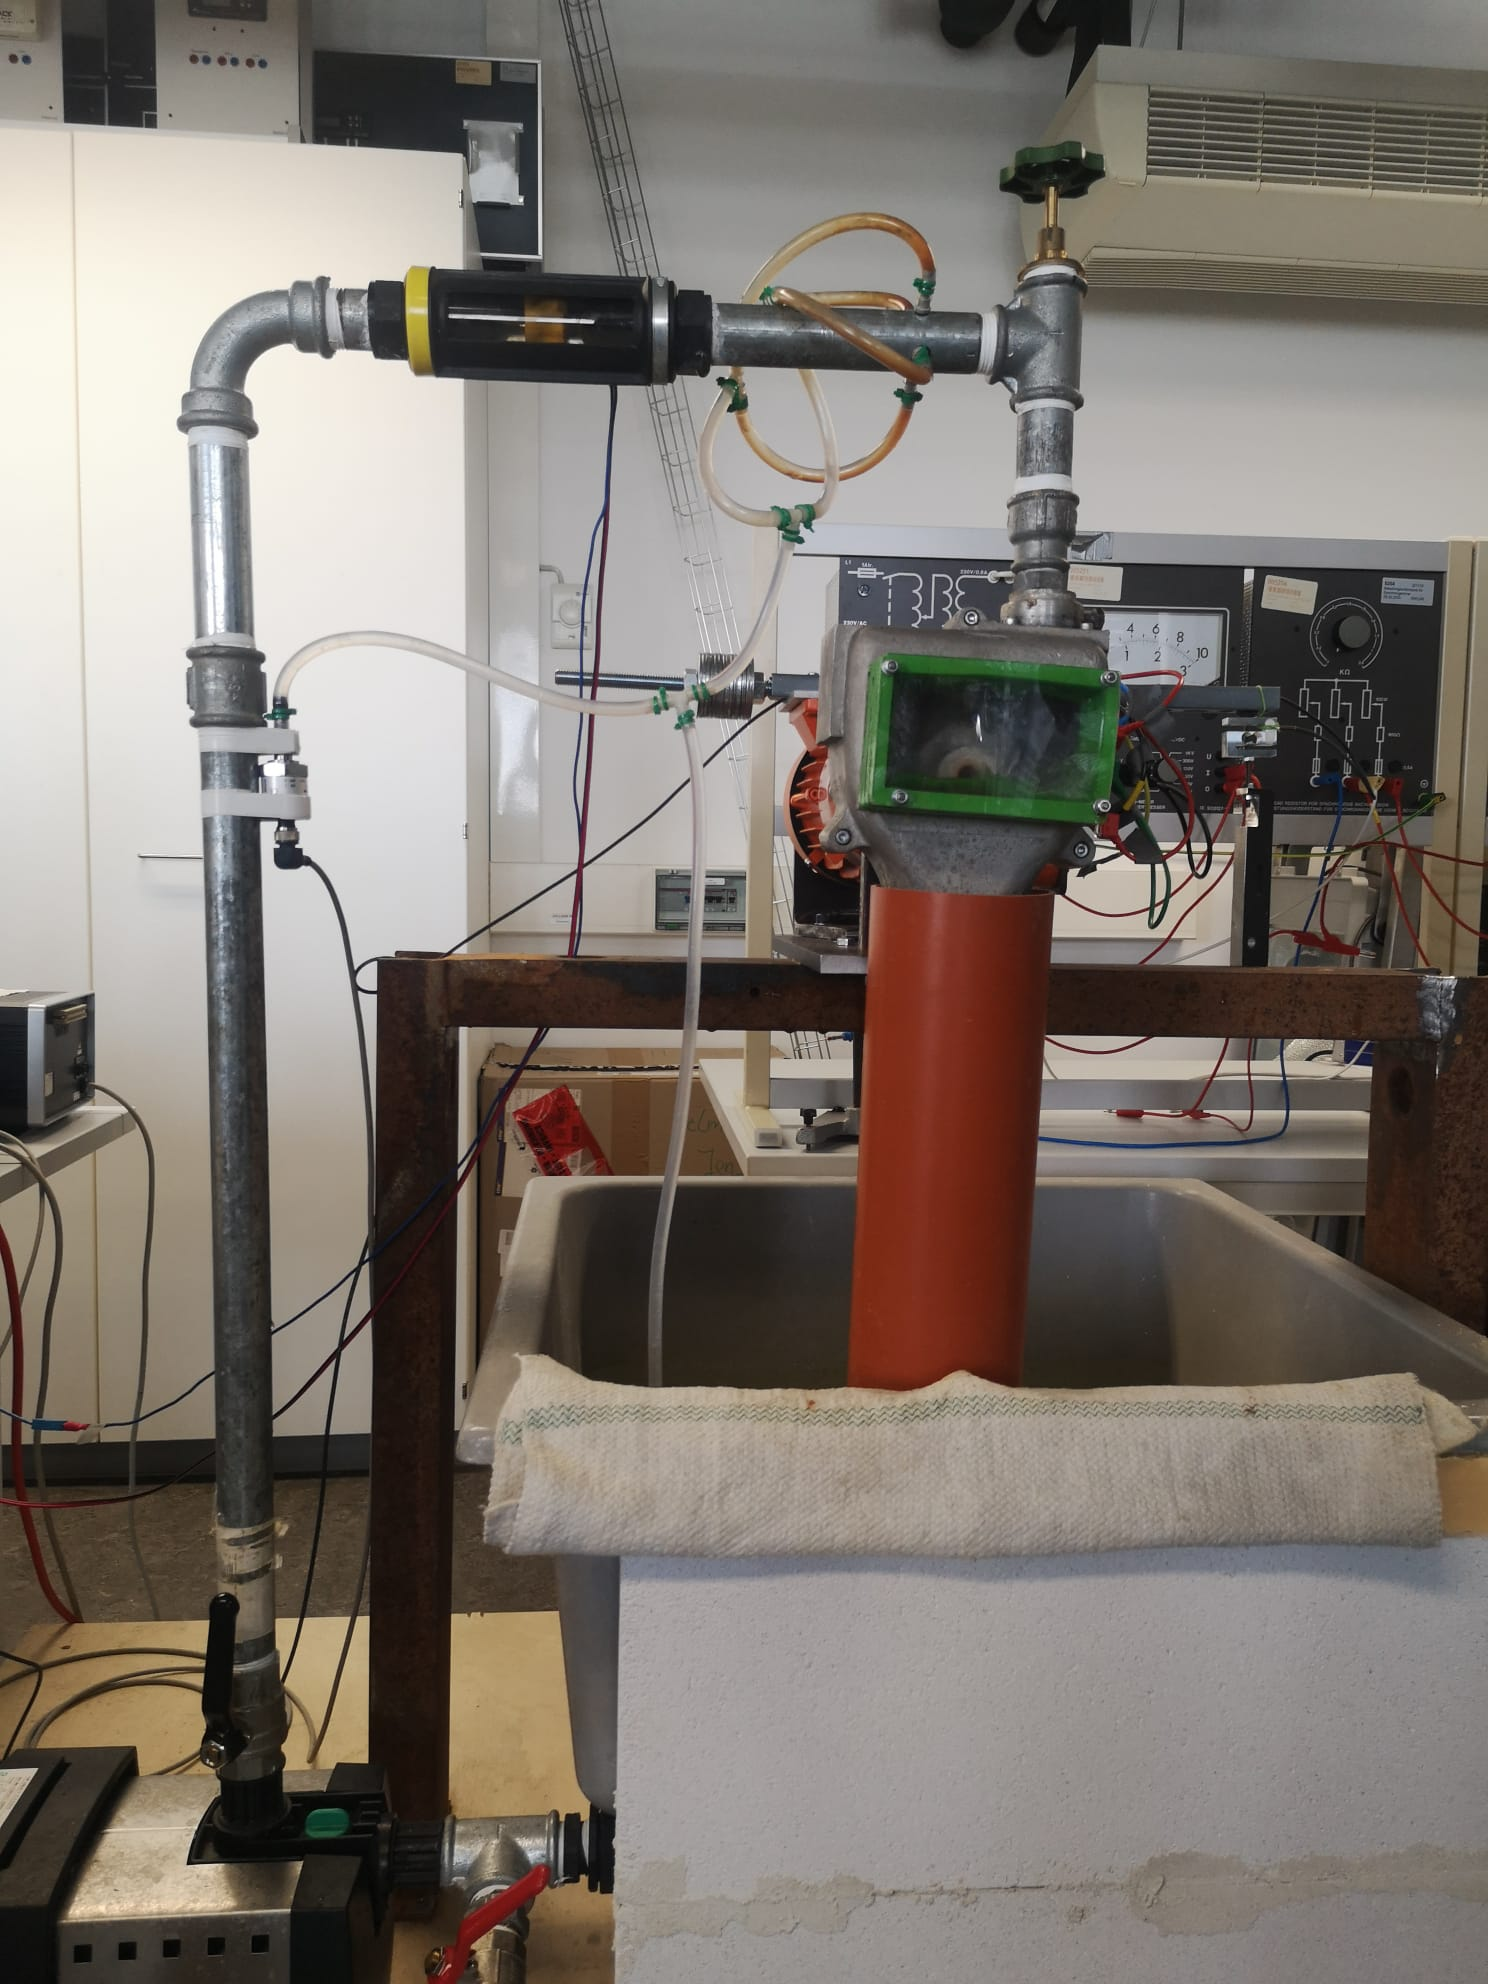
\includegraphics[scale=0.125]{Abbildungen/Aufbau Pelton.jpeg}
    \caption{Versuchsaufbau im Stillstand}
    \label{fig:Aufbau_Stillstand}
\end{figure}

An die Achse der Peltonturbine ist zusätzlich ein fremderregter Synchrongenerator mit einstellbarer Last gekoppelt.
An diesem werden die Drehzahl der Turbine mit einem Handmessgerät, sowie die mechanische Belastung am Generator mittels eines Kraftsensors gemessen.\\
Hier werden als Drehzahlmessgerät der \textit{VOLTCRAFT DT-10L} und als Kraftsensor der \textit{ME-Meßsysteme KD40S} verwendet.
Die Draufsicht auf die Kopplung und den Synchrongenerator ist in \autoref{fig:Synchrongenerator} dargestellt.\\

\begin{figure}[H]
    \centering
    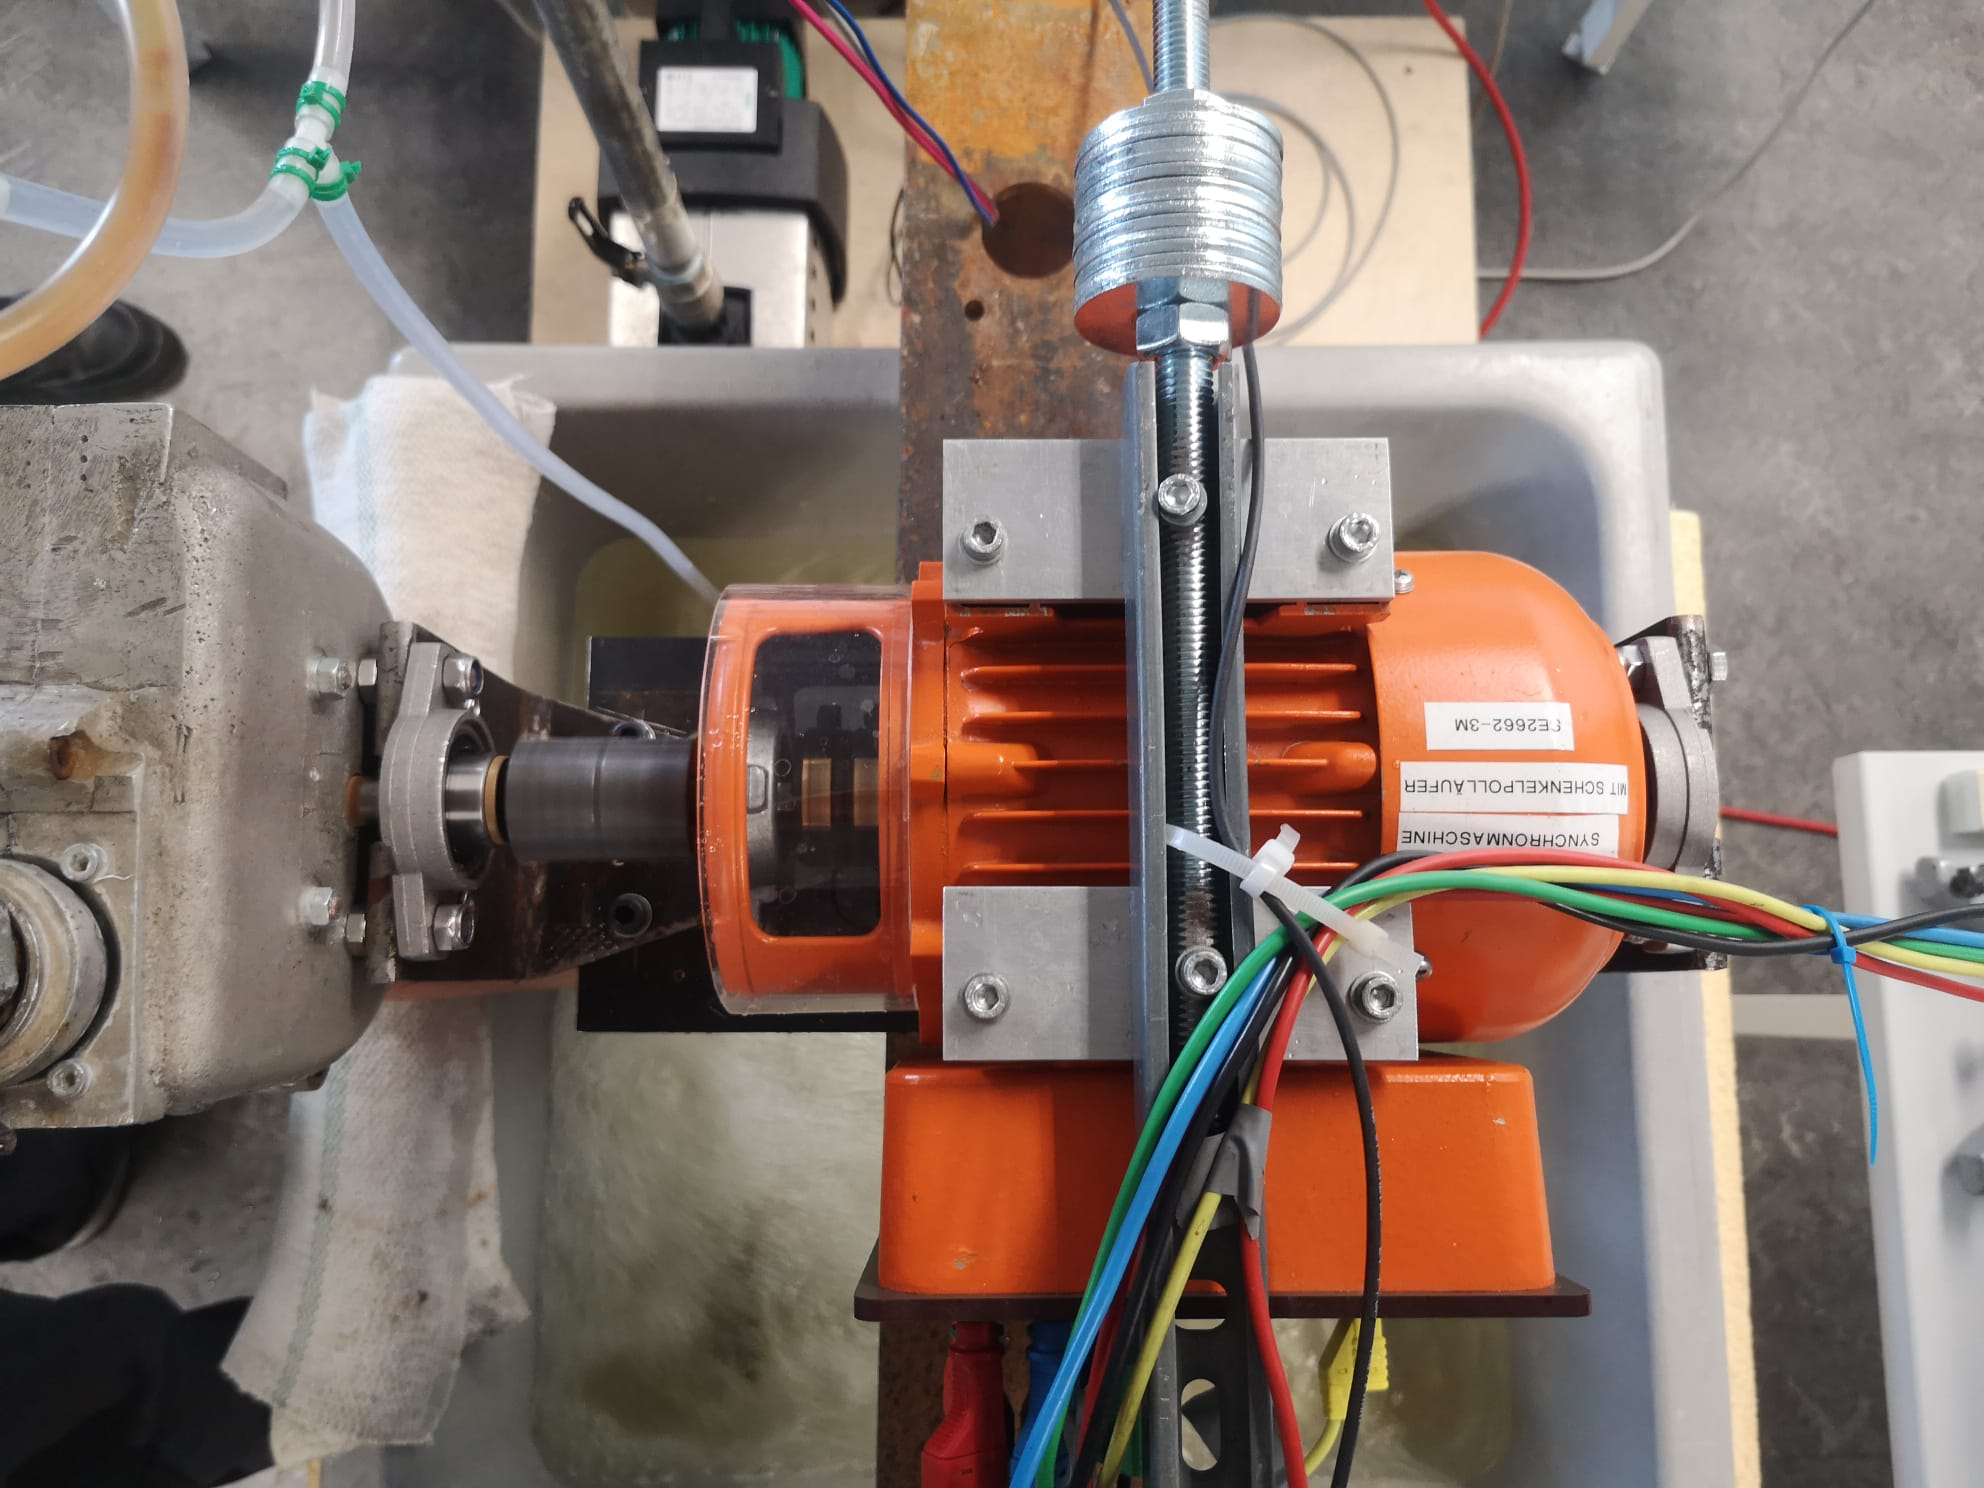
\includegraphics[width=0.5\textwidth]{Abbildungen/Generator.jpeg}
    \caption{Synchrongenerator}
    \label{fig:Synchrongenerator}
\end{figure}

Um den Erregerstrom des Synchrongenerators einstellen und anzeigen lassen zu können ist der Generator in einer Sternschaltung an eine Schalttafel angeschlossen.
Des Weiteren kann an dieser Schalttafel auch der Lastwiderstand eingestellt werden.\\
Zusätzlich werden zwei Multimeter angeschlossen um den Phasenstrom, sowie die Leiterspannung messen zu können.\\
Der gesamte Aufbau der Schalttafel inklusive Multimeter ist in \autoref{fig:Schalttafel} zu sehen.

\begin{figure}[!ht]
    \centering
    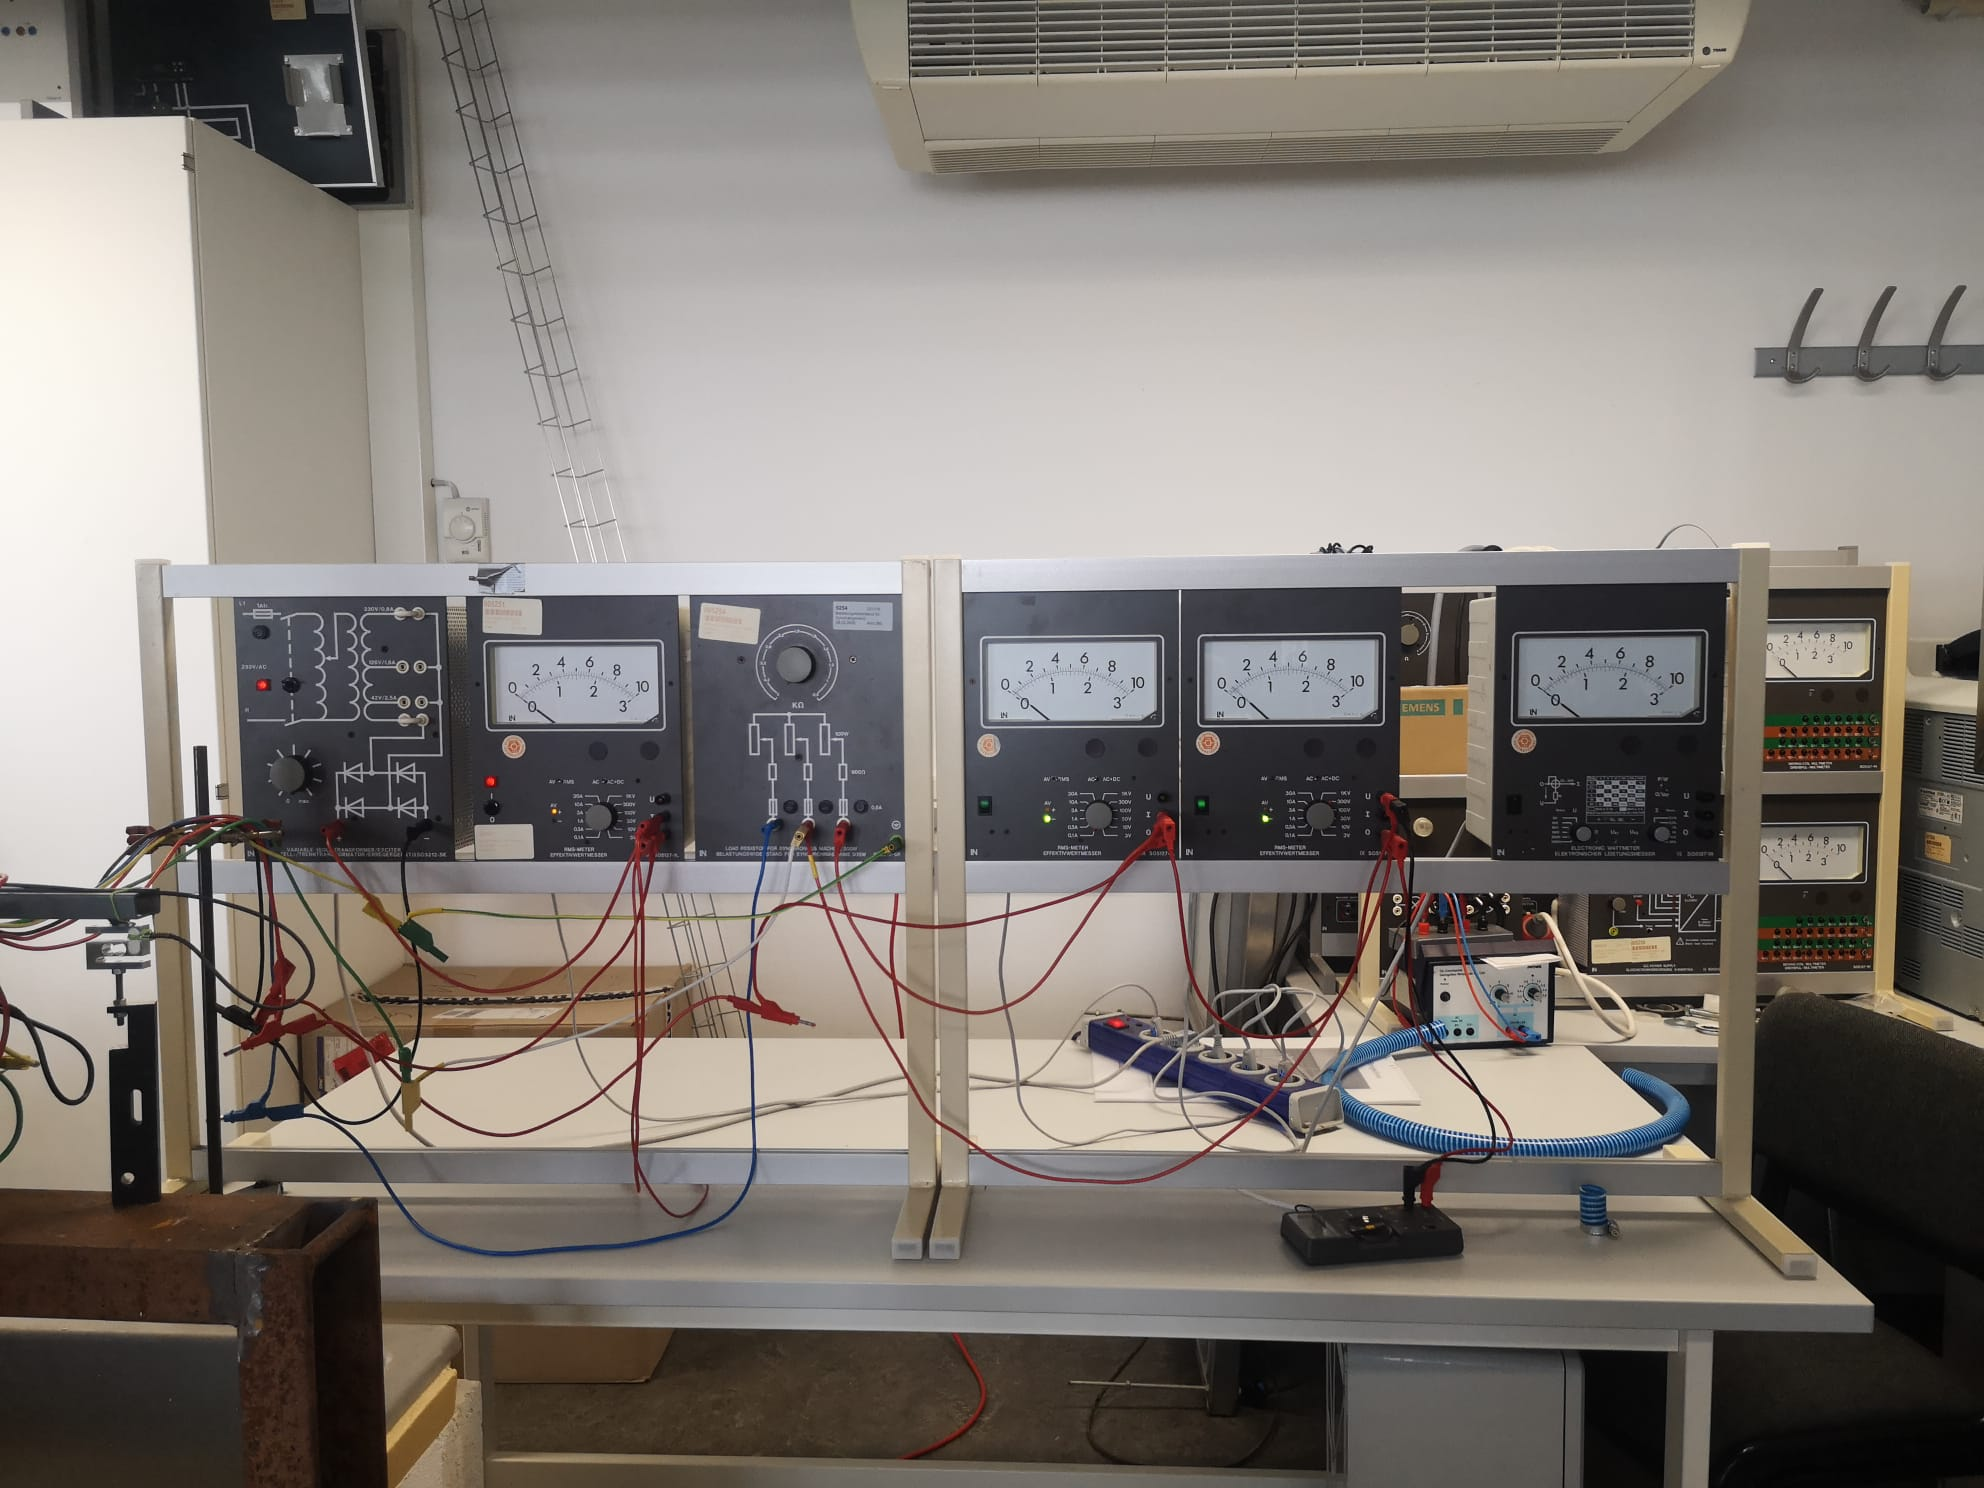
\includegraphics[width=0.5\textwidth]{Abbildungen/Schalttafel.jpeg}
    \caption{Schalttafel}
    \label{fig:Schalttafel}
\end{figure}